% Advanced bioinformatics course - Presentation of February 21st 2012.
%
% The presentation presents the semantic web in general as an evolution
% of the classic web and its use as a data integration plateform for
% bioinformatics.
%

\presentationHead{
    \documentclass[xcolor=dvipsnames]{beamer}
}

\handoutHead{
    \documentclass[handout,xcolor=dvipsnames]{beamer}
}

\mode<handout>{
%%% To generate the handout
\usepackage{handoutWithNotes}

\pgfpagesuselayout{3 on 1 with notes}[a4paper,border shrink=5mm]
% Add border around the first 3 slides in the page
\pgfpageslogicalpageoptions{1}{border code=\pgfusepath{stroke}}
\pgfpageslogicalpageoptions{2}{border code=\pgfusepath{stroke}}
\pgfpageslogicalpageoptions{3}{border code=\pgfusepath{stroke}}
}

\usepackage[utf8]{inputenc}
\usepackage{textcomp}
\usepackage{tikz}

\usetheme{wur}
\setbeamertemplate{navigation symbols}{}
\def\cmd#1{\texttt{\textbackslash #1}}
\def\env#1{\texttt{#1}}

%\title{Literature discussion}
\subtitle{From data integration to semantic integration}
\author{Pierre-Yves Chibon}
\logobartext{21-02-2012}
\institute{Wageningen University - Plant Breeding}

\newlength{\textlarg}
\newcommand{\barre}[1]{%
   \settowidth{\textlarg}{#1}
   #1\hspace{-\textlarg}\rule[0.5ex]{\textlarg}{0.5pt}}


\begin{document}

\whitesheets

\frame{\titlepage}

\section{Introduction}
\frame{
    \frametitle{Overview}
    \begin{itemize}
        \item The web: principles and historic
        \item Data integration on the web
        \item Semantic web technology
    \end{itemize}
    \begin{tikzpicture}[remember picture,overlay]  
    \node [xshift=-3cm,yshift=3cm] at (current page.south east)
        {
\includegraphics[width=5cm]{img/techsupport}};
    \end{tikzpicture}
}

\subsection{The internet}
\frame{
    \frametitle{The internet}
    \begin{center}
    
\includegraphics[width=8cm]{img/internet_cat}
    \end{center}
}

\frame{
    \frametitle{The internet}
    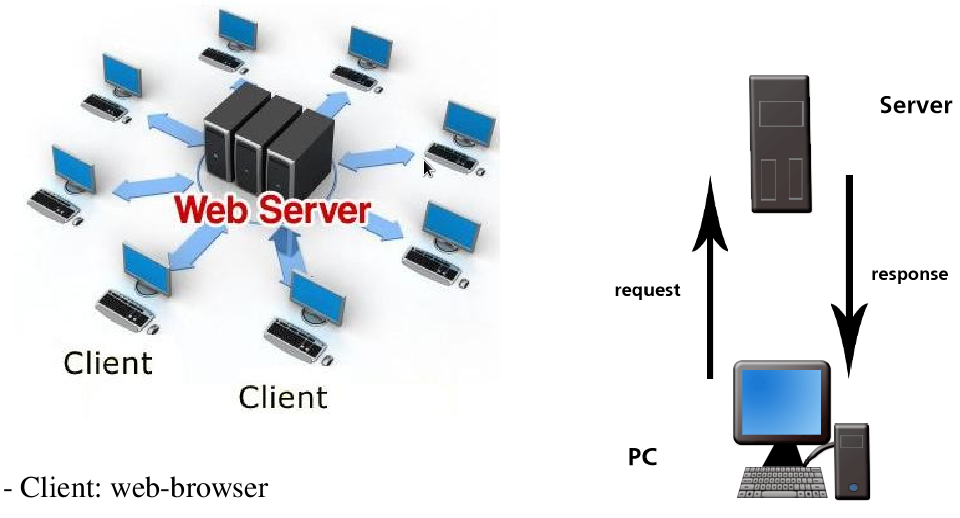
\includegraphics[width=10cm]{img/internet}
}

\frame{
    \frametitle{The internet}
    \begin{itemize}
        \item Simple communication protocole
        \item Client sends a request
        \begin{itemize}
            \item http://localhost/hello.html
        \end{itemize}
        \item Server sends an answer
        \begin{itemize}
            \item html
        \end{itemize}
        \item Client displays this answer \newline
    \end{itemize} 
    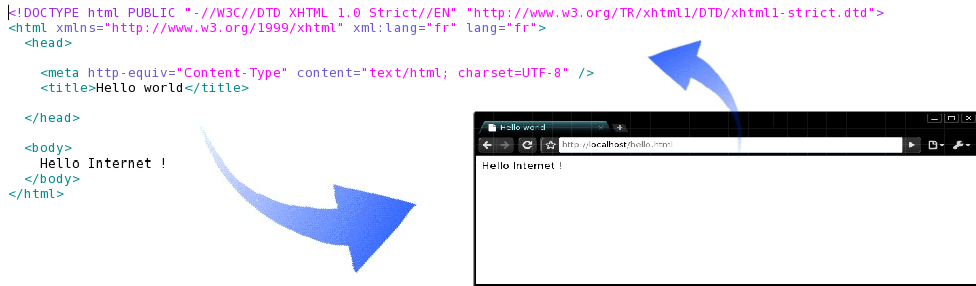
\includegraphics[width=10cm]{img/communication}
}

\subsection{The web}
\frame{
    \frametitle{The web}
    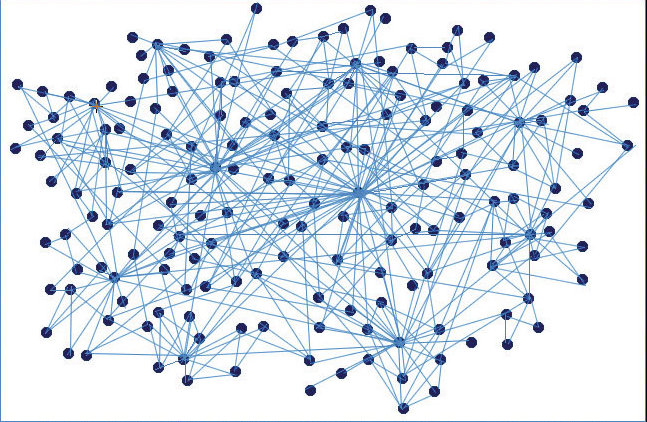
\includegraphics[width=10cm]{img/webmap}\newline
}

\subsubsection{The web 1.0}
\frame{
    \frametitle{The web 1.0}
    \begin{itemize}
        \item Static web
        \item No changes / updates
        \item No interaction with the user
        \item Plain html \newline
    \end{itemize} 
    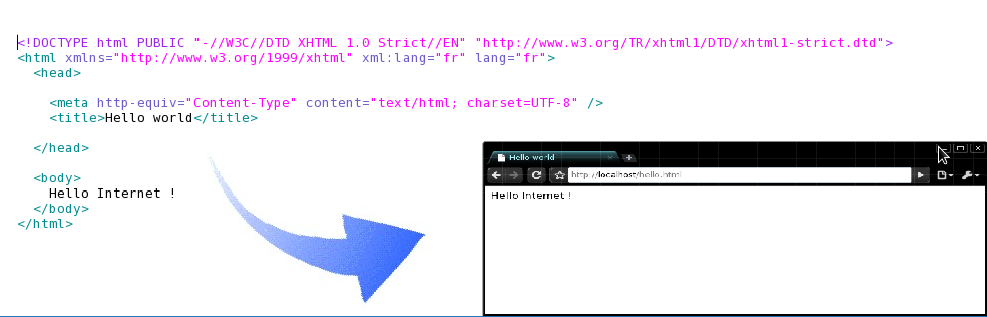
\includegraphics[width=11cm]{img/web1}\newline
}

\subsubsection{The web 2.0}
\frame{
    \frametitle{The web 2.0}
    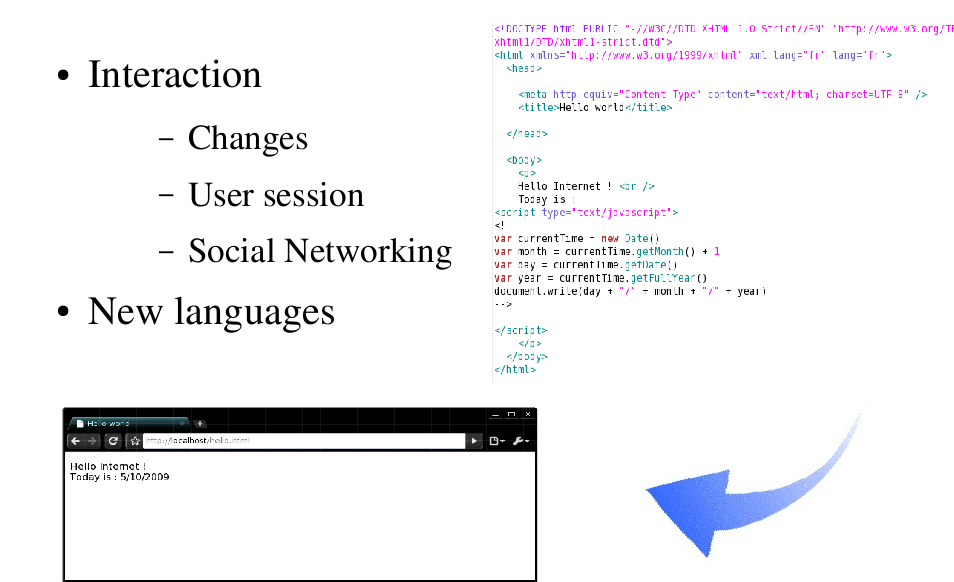
\includegraphics[width=11cm]{img/web2}\newline
}

\frame{
    \frametitle{The web 2.0}
    \begin{itemize}
        \item The web as we know it today
        \item Social network website: facebook, linkedin, viadeo...
        \item CMS / web-log (blog)
        \item google maps, mail, doc, search
        \item wikipedia
        \item ...
    \end{itemize}
    \begin{tikzpicture}[remember picture,overlay]  
    \node [xshift=-3cm,yshift=3cm] at (current page.south east)
        {
\includegraphics[width=5cm]{img/wikipedialol}};
    \end{tikzpicture}
}

\frame{
    \begin{center}
        \huge  What about biology ?
    \end{center}
}

\subsubsection{The web of biology}
\frame{
    \frametitle{The web of biology}
    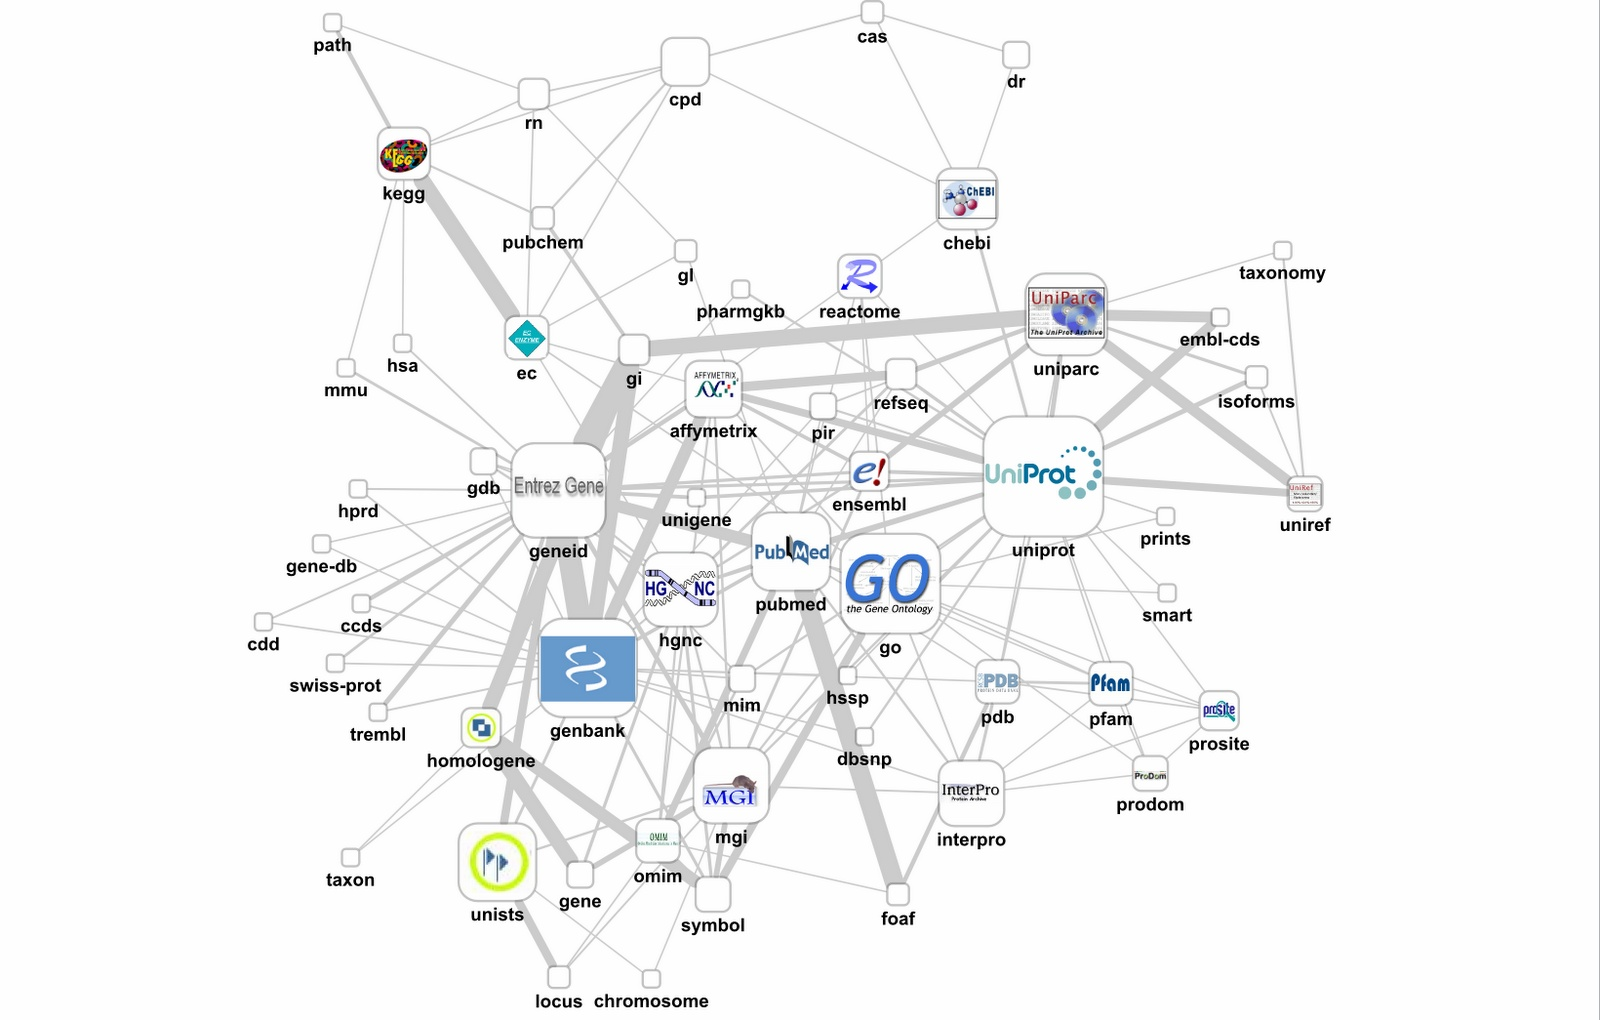
\includegraphics[width=10cm]{img/bio2rdf}\newline
}

\section{Data integration}
\frame{
    \frametitle{Data integration on the web}
    \begin{itemize}
        \item Data warehouse
        \item HTML parsing
        \item Web-services
    \end{itemize}
}

\subsection{Data warehouse}
\frame{
    \frametitle{Data integration : data warehouse}
    \begin{itemize}
        \item Download the database
        \item Generate a giant database with all the information
        \item Needs large resources
        \item High cost in maintainance
        \item Can only be partly automated \newline
        \pause
        \item Not always possible...
        \begin{itemize}
            \item Access
            \item License
        \end{itemize}
    \end{itemize}
}

\frame{
    \frametitle{Data integration on the web}
    \begin{itemize}
        \item \barre{Data warehouse}
        \item HTML parsing
        \item Web-services
    \end{itemize}
}

\subsection{HTML parsing}
\frame{
    \frametitle{Data integration : HTML parsing}
    \begin{itemize}
        \item Retrieve the plain html
        \item Extract programmatically

        information from it \newline
        \pause
        \item make sense of the mess \newline
        \item HTML can be ugly!
    \end{itemize}
}

\frame{
    \frametitle{Data integration : HTML parsing}
    Facebook:
    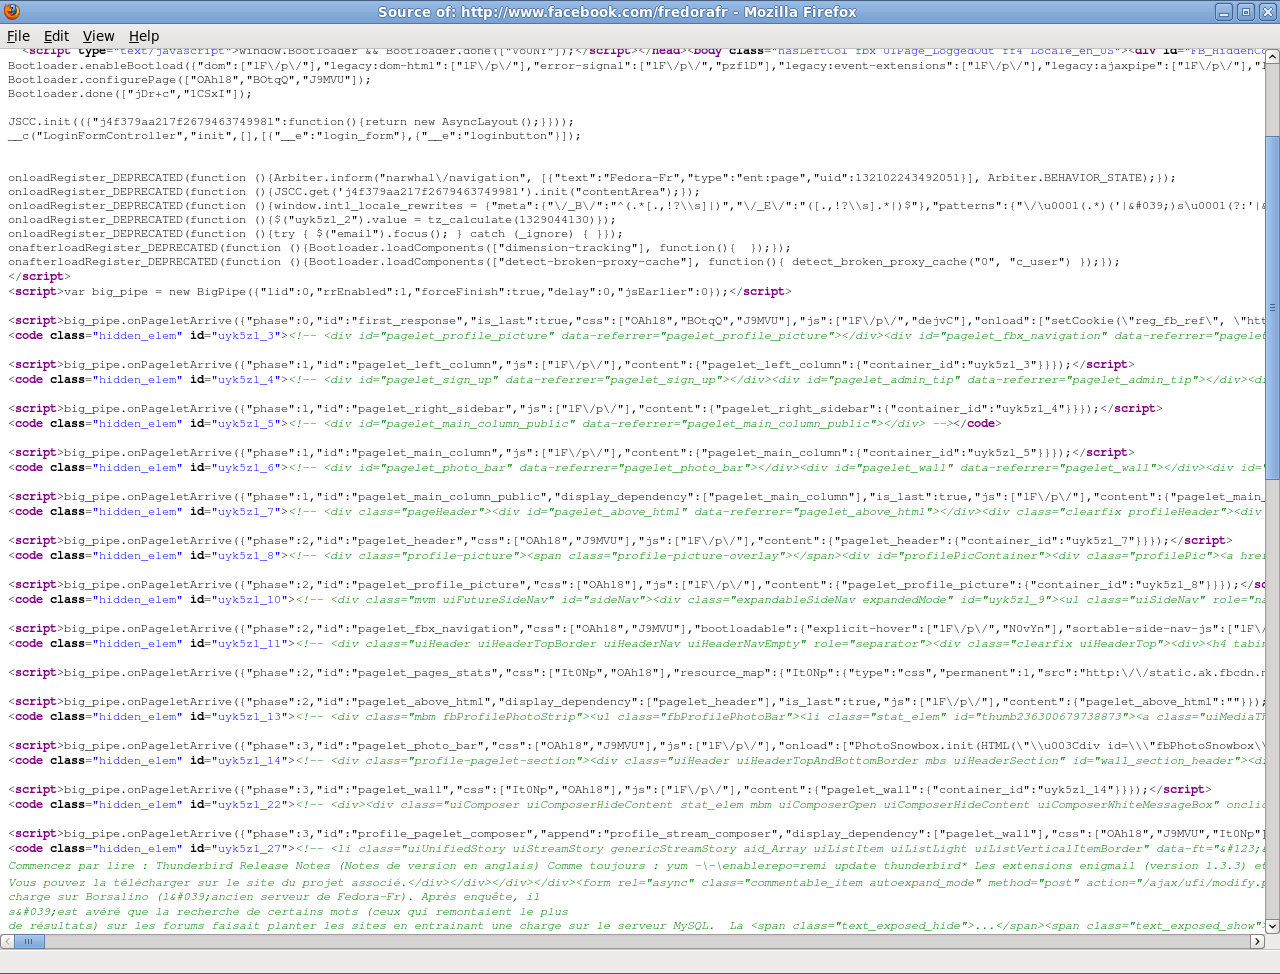
\includegraphics[width=11cm]{img/facebook}\newline
}

\frame{
    \frametitle{Data integration : HTML parsing}
    Linkedin:
    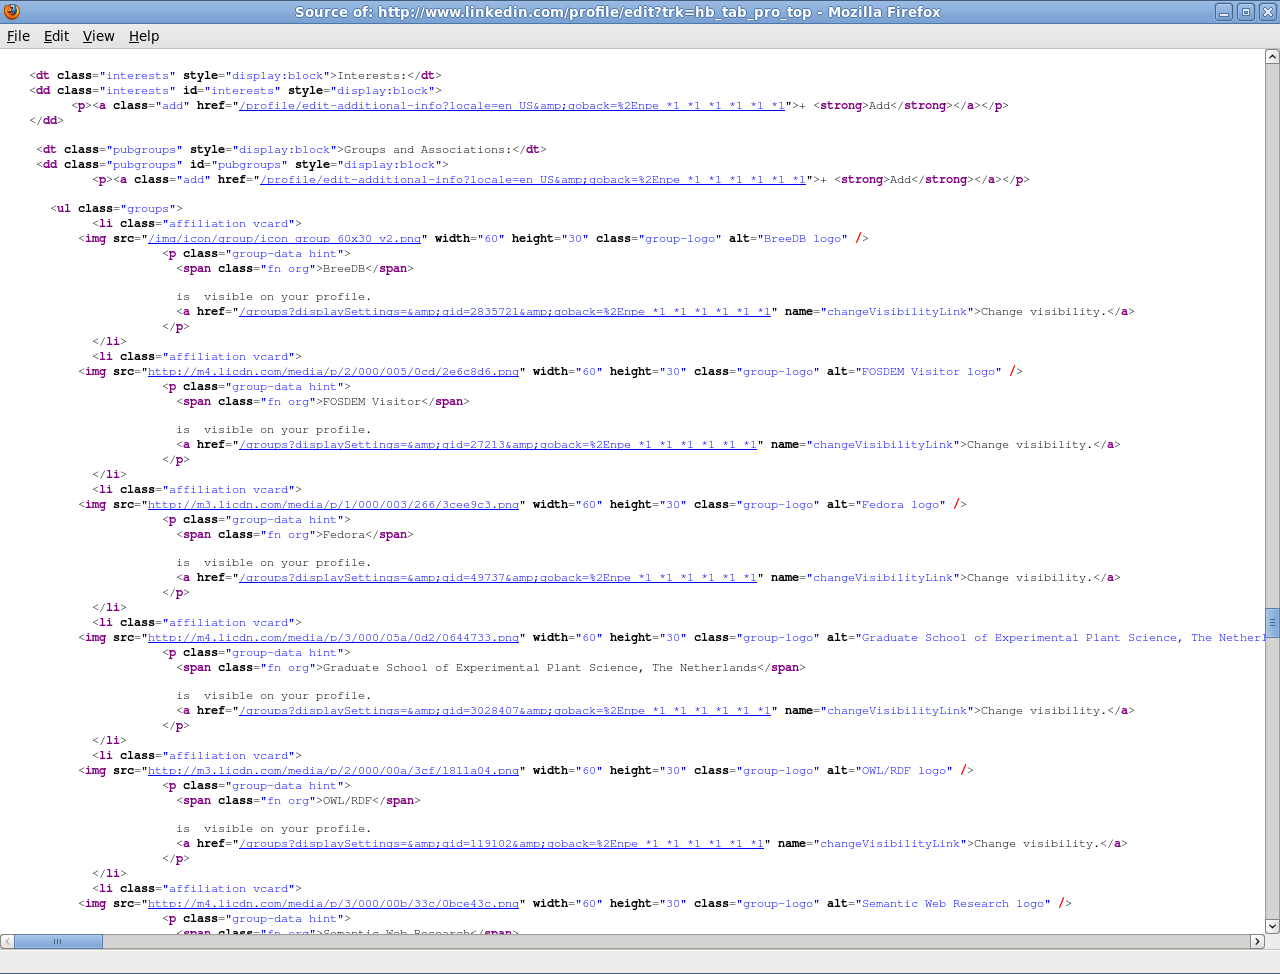
\includegraphics[width=11cm]{img/linkedin}
}

\frame{
    \frametitle{Data integration : HTML parsing}
    \begin{itemize}
        \item One parser per web-site
        \item Parser changes everytime the website changes
        \item Error-prone
        \item If retrieving a lot of information $\rightarrow$ DoS \newline
        \item Not reliable over time
        \item Can not scale
    \end{itemize}
}

\frame{
    \frametitle{Data integration on the web}
    \begin{itemize}
        \item \barre{Data warehouse}
        \item \barre{HTML parsing}
        \item Web-services
    \end{itemize}
}

\subsection{Web-services}
\frame{
    \frametitle{Data integration : web-services}
    \begin{itemize}
        \item Programmatic access to the information
        \item Send xml to a server
        \item Receive xml from the server \newline
        \pause
        \item Retrieve data
        \item Run analysis \newline
        \pause
        \item Chain the services
    \end{itemize}

}

\frame{
    \frametitle{Data integration : web-services}
    \begin{itemize}
        \item Workflow
    \end{itemize}
    \begin{center}
        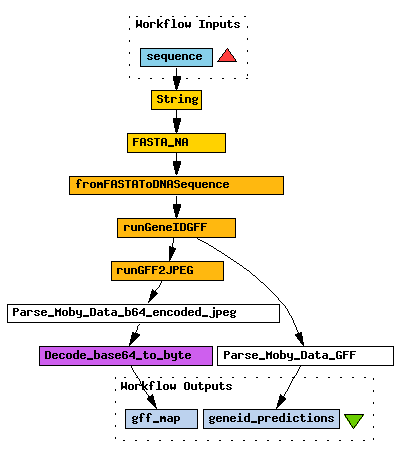
\includegraphics[width=5cm]{img/workflow}
    \end{center}
}

\frame{
    \frametitle{Data integration : web-services}
    Status:
    \begin{itemize}
        \item EBI
        \item KEGG
        \item NCBI
    \end{itemize}
    Basic information retrieval web-services
}

\frame{
    \frametitle{Data integration : web-services}
    \begin{columns}
        \column{0.5\textwidth}
        
\includegraphics[width=2cm]{img/positive}
        \begin{itemize}
            \item No HTML parsing
            \item Latest information
            \item Scale (to a certain point)
            \item Major data provider have adopted them
            \item Allows to delegate large analysis to other resources
            \item No maintainance required (unless the web-service changes)
        \end{itemize}
        \column{0.5\textwidth}
        
\includegraphics[width=2cm]{img/negative}
        \begin{itemize}
            \item Can be hard to find
            \item Unclear as what they do
            \item Needs knowledge wrt to input/output
            \item Use different protocol
            \item Dependence on external services
            \item Security / confidentiallity - your data leaves your computer
        \end{itemize}
    \end{columns}
}

\frame{
    \frametitle{Data integration : web-services}
    Hard to find
    \begin{center}
        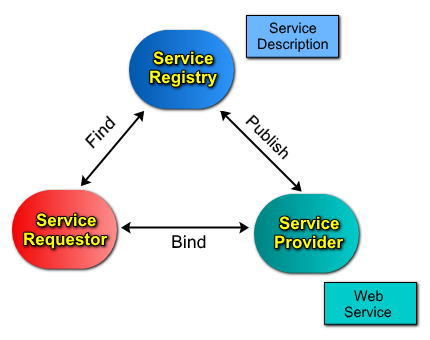
\includegraphics[width=6cm]{img/wsarchitecture}
    \end{center}
    \begin{itemize}
        \item http://www.biocatalogue.org/
        \item http://biomoby.org/
    \end{itemize}
}

\frame{
    \frametitle{Data integration : web-services}
    \begin{itemize}
        \item BioMoby
    \end{itemize}
    \begin{center}
        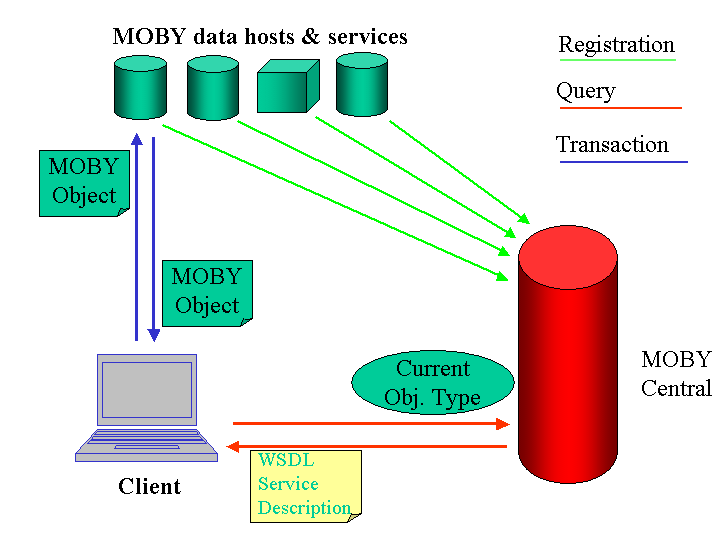
\includegraphics[width=8cm]{img/moby}
    \end{center}
}

\frame{
    \frametitle{Data integration on the web}
    \begin{itemize}
        \item \barre{Data warehouse}
        \item \barre{HTML parsing}
        \item \barre{Web-services} ?
    \end{itemize}
    \begin{tikzpicture}[remember picture,overlay]
    \node [xshift=-3cm,yshift=3cm] at (current page.south east)
        {
\includegraphics[width=5cm]{img/sad}};
    \end{tikzpicture}
}

\section{The semantic web}
\frame{
    \frametitle{Web 3.0: the semantic web}
    \begin{itemize}
        \item Add meaning to the web
        \item Machine readable
        \item Integrative
    \end{itemize}
    \begin{tikzpicture}[remember picture,overlay]
    \node [xshift=-3cm,yshift=3cm] at (current page.south east)
        {
\includegraphics[width=5cm]{img/surprise_chicken}};
    \end{tikzpicture}
}

\subsection{The semantic web - The basis of the web 3.0}
\frame{
    \frametitle{Web 3.0: the semantic web - The basis}
    \begin{itemize}
        \item Add meaning to the web
    \end{itemize}
    \begin{center}
        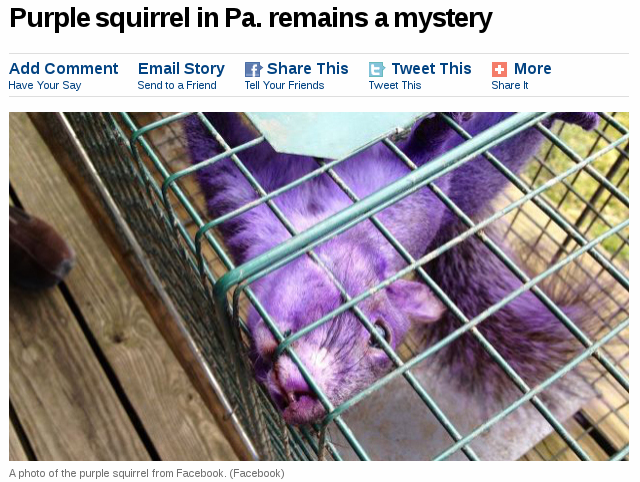
\includegraphics[width=8cm]{img/purplesquirrel}
    \end{center}
    \small (No squirrel has been harmed in the realization of this presentation)
}

\frame{
    \frametitle{Web 3.0: the semantic web - The basis}
    Human
    \begin{itemize}
        \item Squirrel is purple
    \end{itemize}
    \pause
    Computer:
    \begin{itemize}
        \item Squirrel is purple \newline{}
        \pause
        \item Squirrel ??
        \item purple ??
    \end{itemize}
    \begin{tikzpicture}[remember picture,overlay]
    \node [xshift=-3cm,yshift=3cm] at (current page.south east)
        {
\includegraphics[width=5cm]{img/omg_wtf}};
    \end{tikzpicture}
}

\frame{
    \frametitle{Web 3.0: the semantic web - The basis}
    \begin{tikzpicture}[remember picture,overlay]
    \node [xshift=-3cm,yshift=-2cm] at (current page.north east)
        {
\includegraphics[width=5cm]{img/spo}};
    \end{tikzpicture}
    \begin{itemize}
        \item Use triples:
        \begin{itemize}
            \item Subject $\rightarrow$ Squirrel
            \item Predicate $\rightarrow$ is
            \item Object $\rightarrow$ Purple \newline
        \end{itemize}
        \pause
        \begin{itemize}
            \item Subject $\rightarrow$ Squirrel
            \item Predicate $\rightarrow$ is
            \item Object $\rightarrow$ Mammalia \newline
        \end{itemize}
        \pause
        \begin{itemize}
            \item Subject $\rightarrow$ Mammalia
            \item Predicate $\rightarrow$ is
            \item Object $\rightarrow$ Animal \newline
        \end{itemize}
        \pause
        \begin{itemize}
            \item Subject $\rightarrow$ Purple
            \item Predicate $\rightarrow$ is
            \item Object $\rightarrow$ color \newline
        \end{itemize}
    \end{itemize}
}

\frame{
    \frametitle{Web 3.0: the semantic web}
    \begin{itemize}
        \item Add triples to the web \newline{}
        \item Associate terms with concepts
        \item Concepts are clearly defined
        \item Concepts are identified by URI
    \end{itemize}
    How do you use the semantic web ?
    \begin{itemize}
        \item Publish data in a semantic format
        \item Annotate your HTML
    \end{itemize}
}

\subsection{Semantic data}
\frame{
    \frametitle{Semantic web : data}
    Uniprot:
    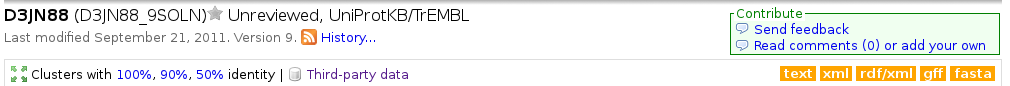
\includegraphics[width=11cm]{img/uniprot}\newline
    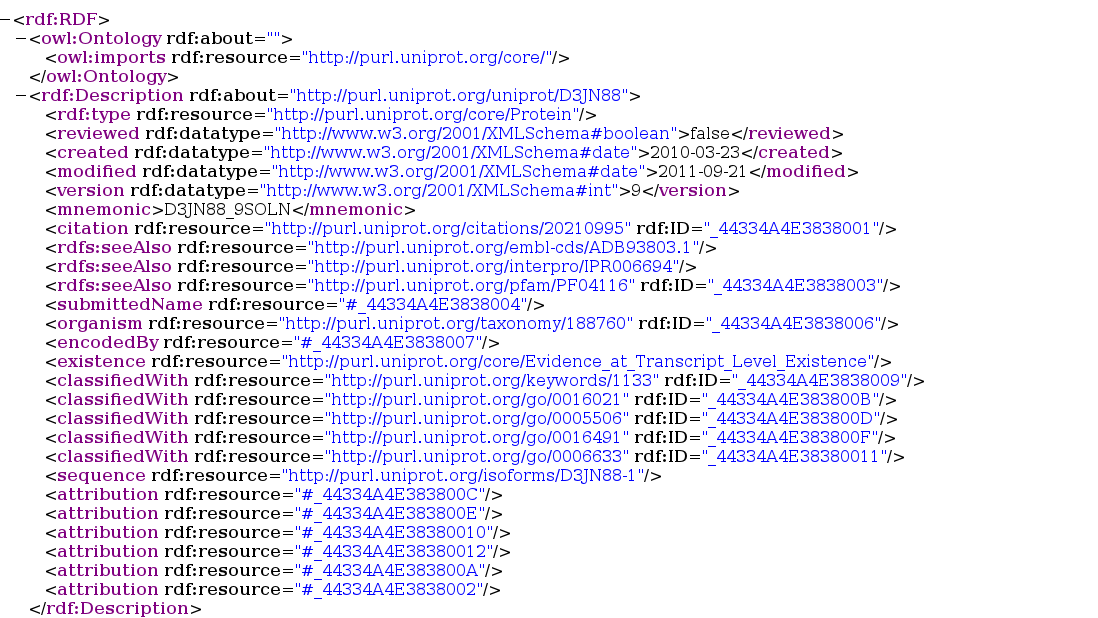
\includegraphics[width=11cm]{img/uniprot2}\newline
}

\frame{
    \frametitle{Semantic web : data}
    Linkedin:
    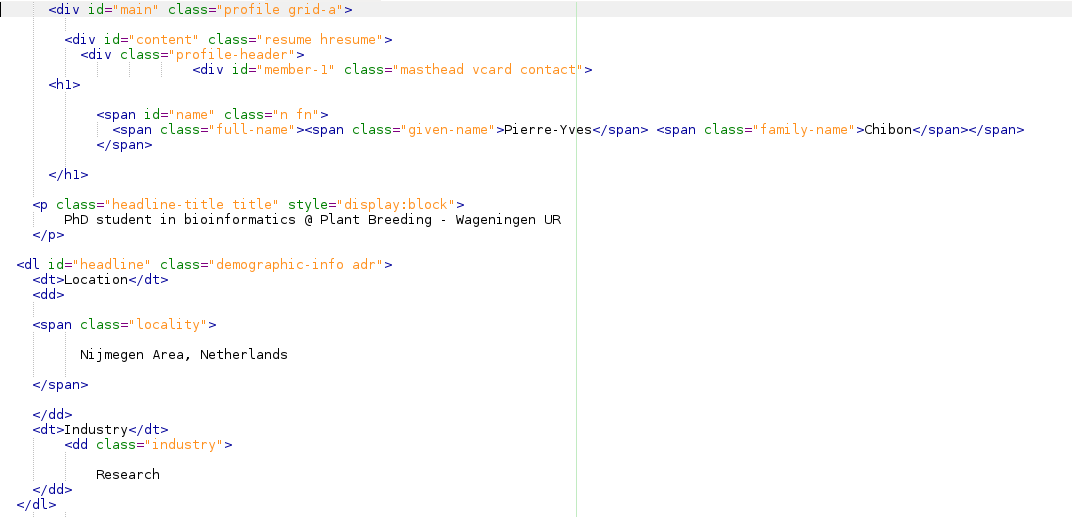
\includegraphics[width=11cm]{img/linkedin2}
}

\frame{
    \frametitle{Semantic web : data}
    Linkedin:
    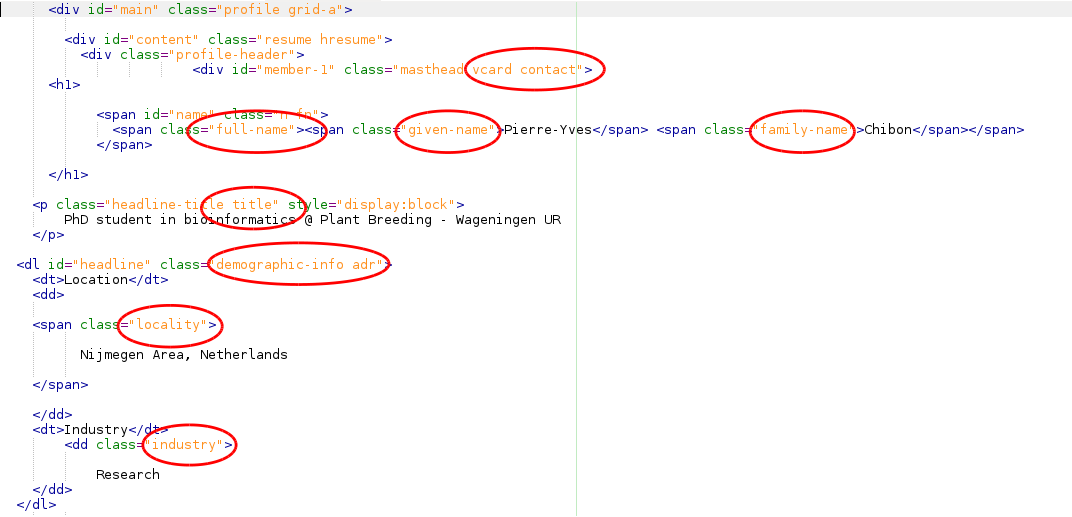
\includegraphics[width=11cm]{img/linkedin3}
}

\section{Conclusions}
\frame{
    \frametitle{Conclusions}
    \begin{itemize}
        \item Designed for data integration
        \item Several formats but no dedicated protocol
        \item Old idea but reaching out
        \item EBI available in RDF \newline
        \item Futur of the (Bio)web ?
    \end{itemize}
}

\frame{
    \frametitle{Conclusions}
    
\includegraphics[width=11cm]{img/threelittlepigshouses}
}

\frame{
    \frametitle{Conclusions}
    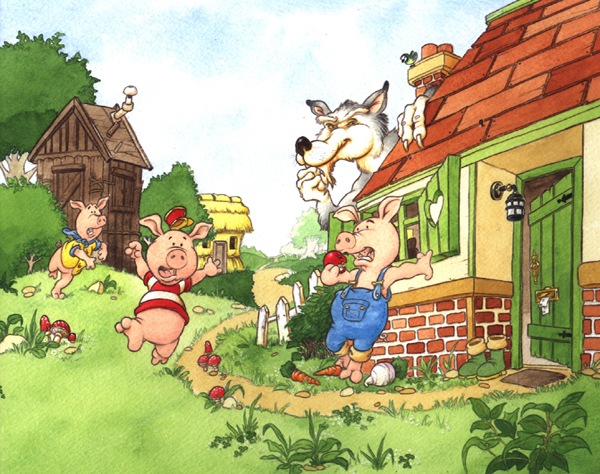
\includegraphics[width=11cm]{img/threelittlepigs}
}

\section{Questions ?}
\frame{
    \frametitle{Questions ?}
    Thank you for your attention.
    \begin{center}
        
\includegraphics[width=8cm]{img/question}
    \end{center}
}

\section{What is what in the semantic web ?}
\frame{
    \frametitle{What is what ?}
    \begin{itemize}
        \item Ontology : Sort of dictionnary standardizing concepts and
        linking them.
        \item RDF/xml, N3, Ntriple, Turtle : format used to represent the
        data semantically.
        \item SPARQL : Query language specific to semantic format
        \item Triple store: Database for semantic data.
        \item URI: Unique Resource Identifier : unique identifier for a
        concept. They can be URL (web address).
    \end{itemize}
}

\end{document}
